\documentclass[12pt]{book}
\usepackage[english]{babel}
\usepackage{natbib}
\usepackage{url}
\usepackage[utf8x]{inputenc}
\usepackage{amsmath}
\usepackage{graphicx}
\graphicspath{{images/}}
\usepackage{parskip}
\usepackage{fancyhdr}
\usepackage{vmargin}
\usepackage{array}
\usepackage{tabularx}
\usepackage{caption}
\usepackage{algorithm}
\usepackage{algpseudocode}
\usepackage{titlesec}% http://ctan.org/pkg/titlesec

\setmarginsrb{3 cm}{2.5 cm}{3 cm}{2.5 cm}{1 cm}{1.5 cm}{1 cm}{1.5 cm}

\title{Assignment}								% Title
\author{A.E Bank \newline N. Blundell}
\date{\today}											% Date

\makeatletter
\let\thetitle\@title
\let\theauthor\@author
\let\thedate\@date
\makeatother

% \pagestyle{fancy}
\fancyhf{}
\cfoot{\thepage}

\begin{document}

%%%%%%%%%%%%%%%%%%%%%%%%%%%%%%%%%%%%%%%%%%%%%%%%%%%%%%%%%%%%%%%%%%%%%%%%%%%%%%%%%%%%%%%%%

\begin{titlepage}
	\centering
    \vspace*{0.5 cm}
    
\includegraphics[scale = 0.75]{wits-logo.jpg}\\[1.0 cm]	% University Logo
    \textsc{\LARGE University of the Witwatersrand}\\[2.0 cm]	% University Name
	\textsc{\Large COMS3007}\\[0.5 cm]				% Course Code
	\textsc{\large Machine Learning}\\[0.5 cm]				% Course Name
	\rule{\linewidth}{0.2 mm} \\[0.4 cm]
	{ \huge \bfseries \thetitle}\\
	\rule{\linewidth}{0.2 mm} \\[1.5 cm]

	\begin{minipage}{0.4\textwidth}
		\begin{flushleft} \large
			\emph{Authors:}\\
			\theauthor
			\end{flushleft}
			\end{minipage}~
			\begin{minipage}{0.4\textwidth}
			\begin{flushright} \large
			\emph{Student Numbers:} \\
				604124 \\
				1132328									% Your Student Number
		\end{flushright}
	\end{minipage}\\[2 cm]

	{\large \thedate}\\[2 cm]

	\vfill

\end{titlepage}

%%%%%%%%%%%%%%%%%%%%%%%%%%%%%%%%%%%%%%%%%%%%%%%%%%%%%%%%%%%%%%%%%%%%%%%%%%%%%%%%%%%%%%%%%

\tableofcontents
\pagebreak

%%%%%%%%%%%%%%%%%%%%%%%%%%%%%%%%%%%%%%%%%%%%%%%%%%%%%%%%%%%%%%%%%%%%%%%%%%%%%%%%%%%%%%%%%
\chapter{Introduction}
This is where we put an introduction.
In addition to the assignment requirements, we explore and discuss methods of analysing categorical data.
The Field Guide apparently (it is not free) states that there is no simple rule for determining whether a mushroom from one of these families is edible or not.

\chapter{Background}

\section{Data Set}
The data set used for this assignment is the Mushroom Data Set.\cite{dataset}
It is based on records from The Audubon Society Field Guide to North American Mushrooms.
The samples are from 23 species of the Agaricus and Lepiota Family.
Each sample has 22 attributes and is classified as either poisonous or edible.
The attributes are as follows:
\begin{center}
\begin{tabularx}{\linewidth}{ |l|X| }
\hline
 0. class (targets) & edible = e, poisonous = p \\
 \hline
 1. cap-shape & bell=b, conical=c, convex=x, flat=f, knobbed=k, sunken=s \\
 \hline
 2. cap-surface & fibrous=f, grooves=g, scaly=y, smooth=s \\
 \hline
 3. cap-colour & brown=n, buff=b, cinnamon=c, gray=g, green=r, pink=p, purple=u, red=e, white=w, yellow=y \\ \hline 4. bruises? & bruises=t, no=f \\
 \hline
 5. odor & almond=a, anise=l, creosote=c, fishy=y, foul=f, musty=m, none=n, pungent=p, spicy=s \\ \hline 6. gill-attachment & attached=a, descending=d, free=f, notched=n \\
 \hline
 7. gill-spacing & close=c, crowded=w, distant=d \\ \hline 8. gill-size & broad=b, narrow=n \\
 \hline
 9. gill-colour & black=k, brown=n,buff=b, chocolate=h, gray=g, green=r,orange=o, pink=p, purple=u, red=e, white=w, yellow=y \\
 \hline
 10. stalk-shape & enlarging=e, tapering=t \\ \hline 11. stalk-root & bulbous=b, club=c, cup=u, equal=e, rhizomorphs=z, rooted=r, missing=? \\
\hline
 12. stalk-surface-above-ring & fibrous=f, scaly=y, silky=k, smooth=s \\ \hline 13. stalk-surface-below-ring & fibrous=f, scaly=y, silky=k, smooth=s \\
\hline
 14. stalk-colour-above-ring & brown=n, buff=b, cinnamon=c, gray=g, orange=o, pink=p, red=e, white=w, yellow=y \\
\hline
 15. stalk-colour-below-ring & brown=n, buff=b, cinnamon=c, gray=g, orange=o, pink=p, red=e, white=w, yellow=y \\
\hline
 16. veil-type & partial=p, universal=u \\ \hline 17. veil-colour & brown=n, orange=o, white=w, yellow=y \\ \hline 18. ring-number & none=n, one=o, two=t \\
 \hline
 19. ring-type & cobwebby=c, evanescent=e, flaring=f, large=l, none=n, pendant=p, sheathing=s, z one=z \\
 \hline
 20. spore-print-colour & black=k, brown=n, buff=b, chocolate=h, green=r, orange=o, purple=u, white=w, yellow=y \\
 \hline
 21. population & abundant=a, clustered=c, numerous=n, scattered=s, several=v, solitary=y \\ \hline 22. habitat & grasses=g, leaves=l, meadows=m, paths=p, urban=u, waste=w, woods=d \\
\hline
\end{tabularx}
\captionof{table}{Legend of attributes and symbols}
\end{center}

The dataset contains 8124 samples.

The 'stalk-root' feature has a '?' as one of it's values.
This indicates a missing value for this feature.
2480 samples have missing values for this feature.
Thus, after dropping these samples, the dataset shrinks to 5644 points.\\

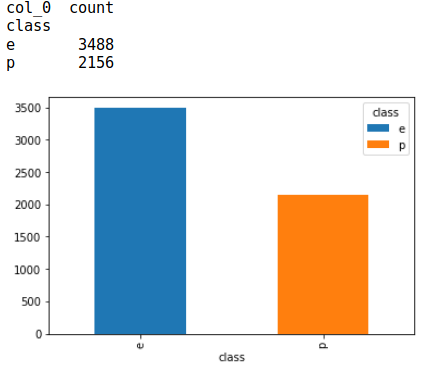
\includegraphics[scale = 0.75]{EvsP.png}\\[1.0 cm]

Below is a sample of the data in it's raw CSV format:\\

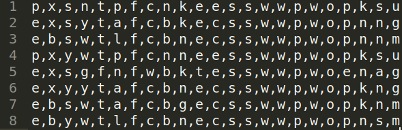
\includegraphics[scale = 0.75]{Rawdata.png}\\[1.0 cm]

\section{Aim}
We will try predicting whether a sample from the dataset is edible or poisonous,
using a Niambh-Bayes Classifier and a Decision Tree Classifier.
We will investigate how using different features, influences
the results.

\section{Pre processing}
All the features in the dataset take on categorical values.
It is interesting to note that no numerically valued features such as 'stem-height'
exist in this data set.\\
Furthermore, features that one may might expect to
take on nemrical values, have been converted to categorical values.\\
We spent a lot of time learning how categorical data is handled.
Before evetually discovering one-hot encoding, we tried learning a method
described in a paper.\cite{RS}
Although the paper gave initial clues as to what to look into,
we soon realised there was not enough time to learn the method. ALthough it relied on concepts we're familiar with,
it required a little more conceptual knowledge to tie it all together.

\subsection{Multiple Correspondence Analysis(MCA)}
We attempted to learn and implement MCA using the Niitsuma paper and a python library called Prince \cite{Prince}
The paper mentioned KL-plots () so we learnt about that.
This lead us to parallel coordinate plots.
We managed to implement one using pandas and got it to look a little nicer using a tutorial\cite{niceParallel}

\subsection{Decision Trees For Feature Analysis}
We note that we could actually use the decision tree algorithm to gain insights into relevant features.
We did infact do this to come up with experiments to run on the dataset.

\subsection{One-Hot Encoding}
One-hot encoding is a procedure where by values that a categorical variable can take on, are converted into
categories themselves.
This allows for analysis to be done on the dataset using conventional plotting methods.

\subsection{Contingency Tables and Bar Graphs}
Using pandas affords us an easy way to get contingency tables and bar graphs.
We can procedururally generate a contingency table or bargraph for any two features.
This can be found in the python notebook:'Decision tree  Learning Pandas  Learning Covariance for categorical vars PCA MCA Regular Simplex Method',
included in the project folder.


\chapter{Algorithms And Experiments}
\section{Algorithms}
\subsection{Naïve-Bayes Classifier}

\begin{algorithm}
\caption{Naïve Bayes}\label{alg:euclid}
\begin{algorithmic}[l]
\Procedure{Get feature counts}{training\_data}\Comment{Training data input}
\For {mushroom in data}
\If {mushroom is edible}
\State {edible\_count++}
\Else
\State {poisonous\_count++}
\EndIf
\For {feature in mushroom}
\State {feature\_counts[feature]++}
\EndFor
\EndFor
\State \textbf{return} {feature\_counts, edible\_count, poisonous\_count}
\EndProcedure
_________________________________________________________________________
\Procedure{Test classifier}{testing\_data}\Comment{Testing data input}

\EndProcedure
\end{algorithmic}
\end{algorithm}



\end{document}

\subsection{Experiments}
The Naive Bayes classifier was tested with Laplace smoothing and without. We also tested it while using the logarithms of the probabilities and while calculating them without using logarithms.
Combinations of these were explored. It was found that the classifier's accuracy was unchanged by the use of logarithms, unless Laplace smoothing was not used. If there
was no Laplace smoothing applied, then the classifier was slightly more accurate (~1%) than the case with Laplace smoothing when logarithms were not used. When logarithms
were calculated, then the use of Laplace smoothing made very little difference (one less misclassification). However, the difference in accuracy across all these cases was no

\section{About this design}
This is a simple report template with the UCT logo. Feel free to use/modify it to suit your needs. Variables that need to be altered have been commented to make modifications easier. For example if you need to change the university logo, look for the comment \texttt{\% University Logo} in this file and then make appropriate modifications in that line.

A Table of Contents and a bibliography have also been implemented. To add entries to your bibliography, simply edit \texttt{biblist.bib} in the root folder and then use the \texttt{\textbackslash cite\{\ldots\}} command in \texttt{main.tex} \cite{bibtex}. The Table of Contents will be updated automatically.

I hope that you find this template both visually appealing and useful.

\hspace{1 cm}--- Lin

\newpage
\bibliographystyle{plain}
\bibliography{biblist}
\end{document}
